\documentclass[a4paper,10pt]{article}
\usepackage{a4wide}
%\documentclass[a4paper,10pt]{scrartcl}
\usepackage[ngerman]{babel}
\usepackage[utf8x]{inputenc}
\usepackage{ulem}
\usepackage{menukeys}
\usepackage{hyperref}

\title{Statistische Zeitreihenanalyse: \\ Brownsche Bewegung, Aktienkurse und Temperaturdaten}
\author{Daniel C. Wagner, Dr. Rudi Schäfer}
\date{März 2015}

\begin{document}
\maketitle


\section{Einleitung}

In diesem Versuch sollen grundlegende Methoden der statistischen Analyse und Beschreibung von Zeitreihen vermittelt und angewandt werden. 
Wir werden dabei drei sehr unterschiedliche Systeme betrachten: die Bewegung von Pollen auf einer Wasseroberfläche, die zeitliche Entwicklung von Aktienkursen, sowie Temperaturzeitreihen. 

Abbildung \ref{fig1} zeigt exemplarisch Zeitreihen der drei genannten Systeme.
Auf den ersten Blick erscheinen alle drei Zeitreihen als ziemlich erratisch oder zufällig. Diese qualitative Beobachtung wollen wir in diesem Versuch präzisieren.

\begin{figure}[htbp]
\begin{center}
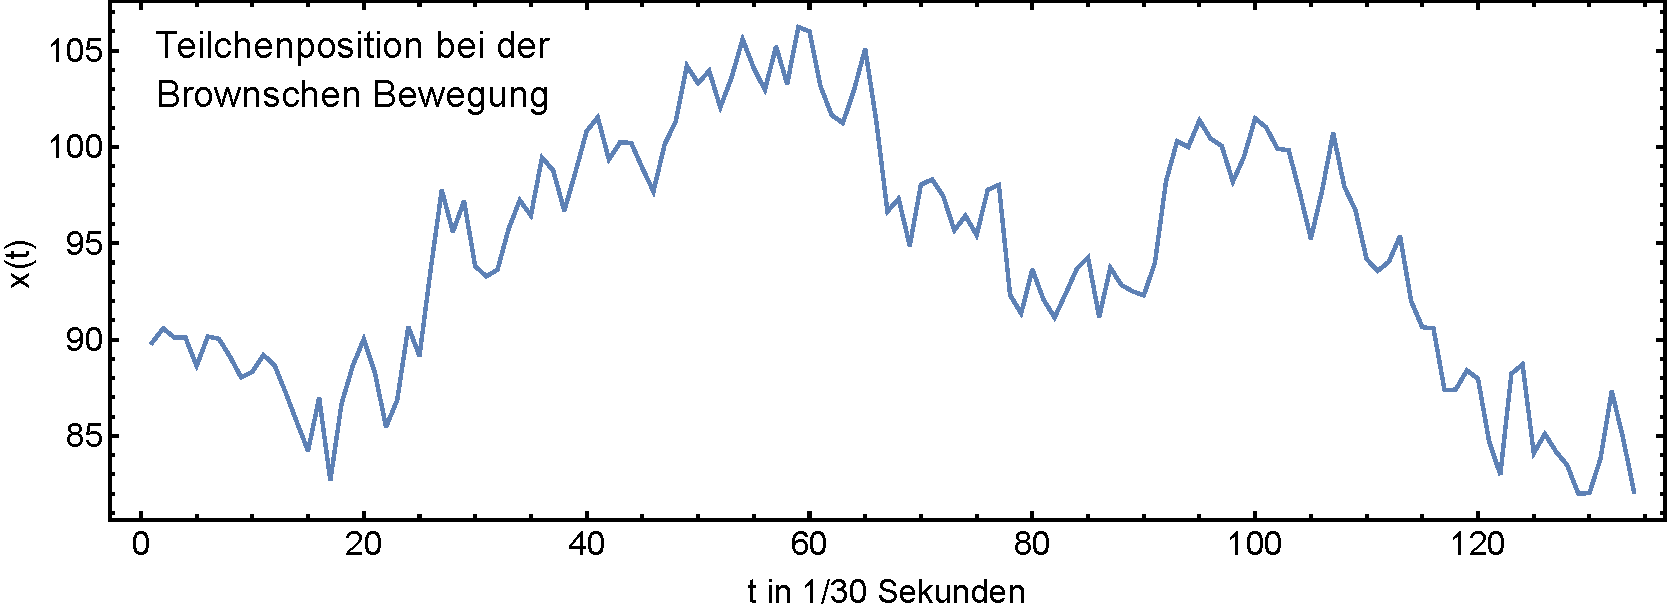
\includegraphics[width=0.6\textwidth]{a1.pdf}\\[1ex]
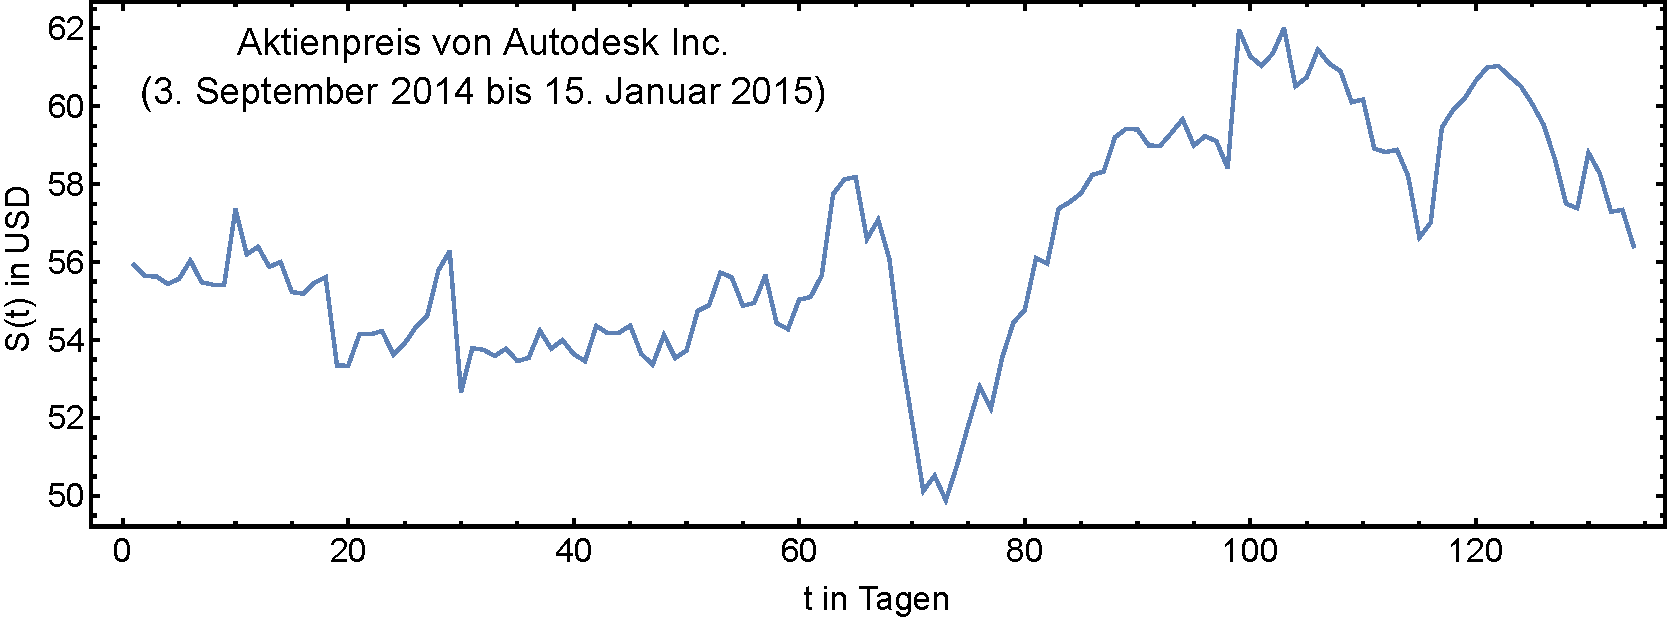
\includegraphics[width=0.6\textwidth]{a2.pdf}\\[1ex]
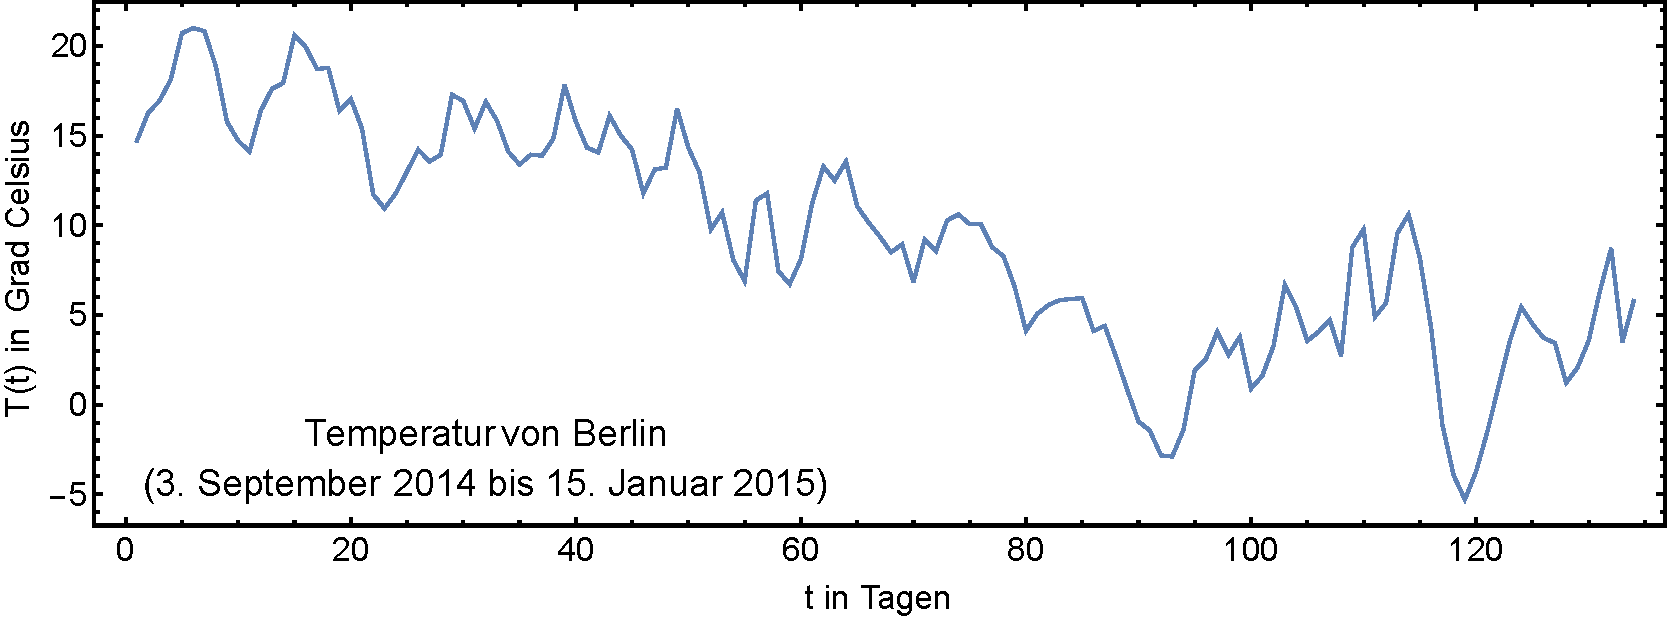
\includegraphics[width=0.6\textwidth]{a3.pdf}
\caption{Beipiele von Zeitreihen für die Brownsche Bewegung (oben), einen Aktienkurs (Mitte), sowie einen Temperaturverlauf (unten).}
\label{fig1}
\end{center}
\end{figure}


\subsection{Brownsche Bewegung}
Der schottische Botaniker Robert Brown beobachtete im Jahre 1827 unter dem Mikroskop, wie Pollen auf einem Wassertropfen unregelmäßig zuckende Bewegungen machten.
Diese Wärmebewegung von Teilchen in Flüssigkeiten und Gasen ist heutzutage nach ihm benannt. Allerdings wurde sie erstmals 1785 von Jan Ingenhousz, einem  niederländischen Arzt und Botaniker, beschrieben. Dieser untersuchte die Bewegung von Holzkohlestaub auf Alkohol. Die Zeitreihen, die man aus solchen Experimenten erhält, sind die in regelmäßigen Abständen aufgezeichneten Positionen der Kohle- bzw. Pollenteilchen (Kolloide).

Obwohl es sich bei einem solchen System um ein rein deterministisches handelt, erscheint die Bewegung völlig erratisch. Sie läßt sich durch einen Zufallsprozess beschreiben [Wiener, Einstein]. Warum ist dem so? Es gibt pro Sekunde eine große Zahl von Stößen zwischen dem Kolloid und den Flüssigkeitsmolekülen (Größenordnung $10^{21}$). Bei jedem dieser Stöße erfährt das Kolloid eine kleine Impulsänderung.
Dies führt effektiv zu einer zufälligen Bewegung des Kolloids. Für die Statistik der Ortsänderungen ergibt sich nach dem zentralen Grenzwertsatz eine Gaußverteilung.
Wir wollen in diesem Versuchsteil ergründen, wie gut empirische Zeitreihen der Kolloidbewegung durch einen Zufallsprozess mit unabhängigen, gaußverteilten Inkrementen beschrieben werden.

% brownsche bewegung, determinisch vs. stochastisch, große zahl, 
% zentraler grenzwertsatz !!!
% Gaußverteilung
% Zufallsbewegung (Wiener Prozess, Einstein)



\subsection{Aktienpreise}
Wie in Abbildung \ref{fig1} zu sehen, sieht auch die zeitliche Entwicklung von Aktienkursen ähnlich erratisch aus wie die Brownsche Bewegung von Kolloiden auf einer Flüssigkeit.
Und tatsächlich hat die Modellierung von Aktienkursen als Zufallsprozess eine lange Tradition, die auf die Doktorarbeit des französischen Mathematikers Louis Bachelier aus dem Jahre 1900 zurückgeht. 
Weshalb aber macht eine solche stochastische Beschreibung für Aktienkurse Sinn, wo doch auf lange Sicht der Aktienkurs das wirtschaftliche Wachstum eines Unternehmens widerspiegeln sollte und die Aktienhändler, die den Preis letztlich bestimmen, auch keineswegs zufällig handeln?
Ersteres führt sicher zu einem deterministischen Anteil, einer sogenannten Drift.
Die Argumentation für den stochastischen Anteil verläuft analog zur Brownschen Bewegung: Obwohl die einzelnen Aktienhändler klare Absichten und Strategien verfolgen, macht die große Vielzahl der Handelsinteraktionen (Größenordnung $10^4$ pro Tag) eine stochastische Modellierung sinnvoll. 

Bachelier nahm für die Änderungen der Aktienpreise in einem festen Zeitintervall eine Gaußverteilung an. 
Dies kann im Modell jedoch einerseits schnell zu negativen Preisen führen, und spiegelt  andererseits nicht den auf längeren Zeithorizonten zu beobachtenden exponentiellen Verlauf der Aktienkurse wieder. 
Um diesen Aspekten gerecht zu werden, nimmt man eine Gaußverteilung für die relativen Preisänderungen (Renditen, englisch: \textit{returns}) an. 
Empirisch ist jedoch seit den 1920er Jahren bekannt, dass Renditeverteilungen in der Regel nicht gaußisch sind, sondern ein stärkeres Gewicht in den Flügeln der Verteilung steckt. Das bedeutet, dass sehr große relative Preisänderungen viel wahrscheinlicher sind, als man von einer Gaußverteilung erwarten würde.
Die einfache Argumentation über den zentralen Grenzwertsatz scheint also bei Aktienkursen nicht zu funktionieren. Die Gründe dafür sind vielfältig und wir werden ihnen im Rahmen dieses Versuchsteils auf den Grund gehen.

% Aktienpreise
% Händler, Preisfindung
% Bachelier
% Preisinkremente, Returns:  im mittel unabhängig, sonst könnte man systematisch gewinn machen
% Nichtstationarität, Volatility clustering
% heavy tails, Risiko (aber auch Chance)



\subsection{Temperaturen}
Das Wetter gilt gemeinhin als Paradebeispiel für chaotische Systeme. 
Gerne wird etwa der Flügel\-schlag eines Schmetterlings in China angeführt, der womöglich so große Auswirkungen haben könne, dass sich das Wetter in Europa änderte. 
Am besten wird die Komplexität der Wetterphänomene jedoch deutlich, wenn man bedenkt, wie außerordentlich schwierig es ist, Vorhersagen zu machen. 
Obwohl die Wetterdienste über die weltweit leistungsstärksten Großrechner verfügen und ein immenser Aufwand in die Messung empirischer Daten, sowie in die Modellbildung fließt, können zuverlässige Vorhersagen oft nur für wenige Tage gemacht werden.

Wir werden uns hier auf Temperaturdaten beschränken. Auch diese zeigen auf den ersten Blick ein recht erratisches Verhalten, siehe Abbildung \ref{fig1}. Jedoch wird es sicher auch starke räumliche und zeitliche Korrelationen im Temperaturverlauf geben, sowie eine starke Abhängigkeit von der Tages- und Jahreszeit.
In diesem Versuchsteil wollen wir diese systematischen Aspekte, sowie den stochastischen Anteil näher ergründen.


% Temperaturdaten
% Wetter als typisches Beispiel chaotischer Systeme
% Sensitivität auf Anfangsbedingungen, bzw. Störungen pflanzen sich nichtlinear fort
% zeitliche und räumliche Korrelationen
% starke Säsonalität im Tages-, sowie Jahresverlauf



\subsection{Vorbereitung, Literatur}

Machen Sie sich mit den Grundbegriffen der Statistik vertraut. 
Orientieren Sie sich dazu an den folgenden Leitfragen:
\begin{itemize}
\item Was versteht man unter Verteilung? 
\item Was ist eine Wahrscheinlichkeitsdichte?
\item Wie schätzt man eine Wahrscheinlichkeitsdichte aus empirischen Daten?
\item Wie ist die Gaußverteilung definiert?
\item Was besagt der zentrale Grenzwertsatz? 
\item Welche Voraussetzungen müssen für den zentralen Grenzwertsatz gelten?
\item Wie misst man statistische Abhängigkeiten zwischen empirischen Zeitreihen?
      (Korrelationskoeffizient, Copula)
\item Was versteht man unter einer Autokorrelationsfunktion?
\item Was ist ein Markov-Prozess?
\item Wie testet man die Markov-Eigenschaft von empirischen Zeitreihen?
\end{itemize}

\vspace*{1cm}
Für einen schnellen Einstieg in diese grundlegenden Fragen eignet sich ein Blick in Wikipedia, sowie die folgende Literatur:

\begin{enumerate}
\item Ulrich Krengel (2005) Einführung in die Wahrscheinlichkeitstheorie und Statistik, Vieweg+Teubner Verlag.
\item Rudi Schäfer (2015) Introduction to copulas: Studying statistical dependencies, Semesterapparat. Siehe hierzu auch den \href{https://aglorke.uni-due.de/fp2/info/For\%20experiment\%201.12\%20-\%20introduction_to_copulas.pdf}{Infotext} auf der Homepage des Praktikums.

\end{enumerate}


% Verteilungen, Gaußverteilung, zentraler Grenzwertsatz
% Markov-Prozess, statistische Unabhängigkeit
% Statistische Abhängigkeiten
%  Korrelationen
%  Copulas
% Autokorrelationsfunktion (gängig zur Prüfung der Markov-Eigenschaft)





% statistische Analyse
% stochastische Modellierung
% stochastische und determinsitsche Aspekte
% zentraler Grenzwertsatz und seine Grenzen
% nicht-stationarität
% nicht-markovsche Eigenschaften
% Gleichgewicht vs. Nichtgleichgewicht

% A random walk down wall street

%\vspace*{1cm}
\newpage

\section{Daten und Auswertung}
Wir werden Sie Schritt für Schritt durch die Auswertung Ihrer Ergebnisse führen. Die Verwendung von Wolfram Mathematica 10, dessen Befehle in dieser Anleitung in \texttt{Schreibmaschinenschrift} gedruckt werden, ist dabei obligatorisch. Es ist oftmals eine Vereinfachung, \texttt{Map} bzw. \texttt{/@} zu nutzen. Zudem werden sogenannte \textit{pure functions} (also \texttt{Function} bzw. \texttt{\#} und \texttt{\&}) als bekannt vorausgesetzt. Machen Sie bei der Bearbeitung der Aufgaben ausführlichen Gebrauch von der Mathematica-Hilfe, in der sämtliche Funktionen an vielen Beispielen erläutert werden.

\vspace*{4ex}

\subsection{Brownsche Bewegung}
Zeichnen Sie die Trajektorien der Partikel aus dem Ihnen zur Verfügung gestellten Video auf und exportieren Sie die Ergebnisse. Die statistische Auswertung dieser Daten erfolgt anschließend in Mathematica. %Folgen Sie dann diesen Schritten:
Gehen Sie wie folgt vor:
\begin{enumerate}
 \item Starten Sie das Programm ImageJ und öffnen Sie das Video zur Brownschen Bewegung: \texttt{File} $\Rightarrow$ \texttt{Open} $\Rightarrow$ Datei auswählen
 \item \texttt{Convert to Grayscale} aktivieren $\Rightarrow$ \texttt{OK}
 \item \texttt{Plugins} $\Rightarrow$ \texttt{Mosaic} $\Rightarrow$ \texttt{Particle Tracker 2D/3D} $\Rightarrow$ No 3D data $\Rightarrow$ \texttt{OK} $\Rightarrow$ Warten!
 \item Kalibrierung gemäß \autoref{fig:param} $\Rightarrow$ (\texttt{Preview Detected} $\Rightarrow$) \texttt{OK} \\
 {\footnotesize (Mehr Informationen unter \url{http://mosaic.mpi-cbg.de/ParticleTracker/}.)}
 
\begin{figure}[htbp]
  \centering
  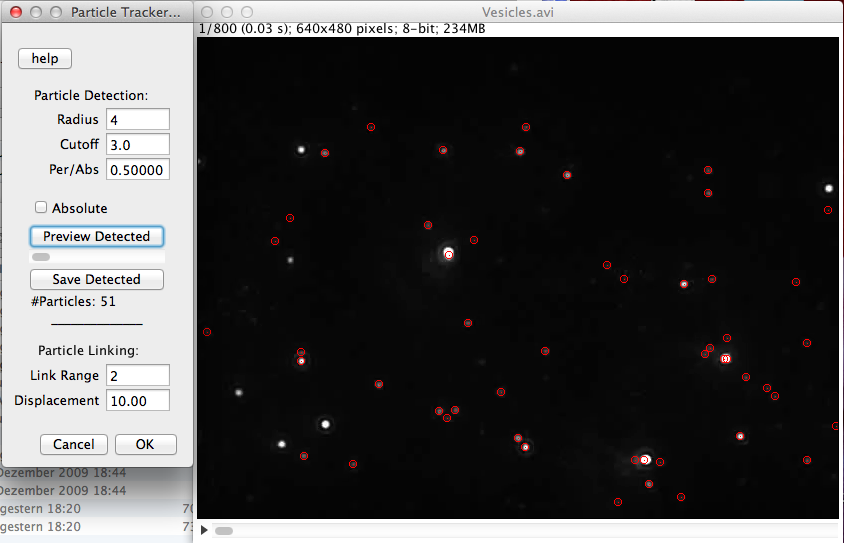
\includegraphics[width=0.8\textwidth]{parameter.png}
  \caption{Paramter für den \textit{particle tracker} für \texttt{Vesicles.avi}.}
  \label{fig:param}
\end{figure}
 
 
% \item Dieser Vorgang kann etwas dauern. Der Fortschritt ist in der Statusleiste des ImageJ-Hauptframes zu sehen.
 \item Im sich öffnenden Fenster \texttt{Results} auf \texttt{All Trajectories to Table} klicken und sie über \texttt{File} $\Rightarrow$ \texttt{Save As} als Tabelle abspeichern.%, die dann in Mathematica 10 zu importieren ist.


 
 \item Lesen Sie die detektierten Trajektorien in Mathematica ein. Nutzen Sie die Funktion \texttt{Import} und importieren Sie die Daten mit den Optionen \texttt{"Data"}, sowie \texttt{"HeaderLines"\ -> 1}. Um nun zwischen den einzelnen Trajektorien separieren zu können, empfehlen wir die Funktion \texttt{Gather}. Alternativ, jedoch viel langsamer, funktioniert dies auch mit \texttt{Select}.
 \item Im Folgenden filtern Sie ungewünschte Trajektorien heraus:
 \begin{itemize}
  \item Berechnen Sie die Anzahl der Zeitschritte für sämtliche Trajektorien und verwerfen Sie jene, die kürzer als $50$ Zeitschritte sind. Benutzen Sie dafür die Funktion \texttt{Delete} bzw. \texttt{Extract} in Verbindung mit \texttt{Position}. \\ \uline{Tipp}: Wenn Sie aus einer Liste \texttt{a} die Positionen aller Werte, die kleiner als \texttt{x} sind, ermitteln möchten, dann lautet ein möglicher Mathe\-matica-Befehl für diese Aufgabe: \texttt{Position[a, \_?(\# < x \&)]}.
  \item Berechnen Sie für alle $M$ übrig gebliebenen Trajektorien die Differenzen (\texttt{Differences}) $\Delta x_n = x_{n+1} - x_{n}$ für $n\in[1,\,L_i-1]$, wenn $L_i$ die Anzahl der Datenpunkte der Trajektorie $i$ ($i\in[1,\,M]$) ist. Wiederholen Sie dies für die zweite Dimension. 
  \item Verwerfen Sie alle Trajektorien, deren Zeitreihen $\Delta x_n$ und/oder $\Delta y_n$ eine zu große Wölbung (\texttt{Kurtosis}) aufweisen. Welche Grenze haben Sie hier gewählt und warum?
  \item Die Anzahl der so gefilterten Trajektorien sei fortan $N$.
 \end{itemize}
 \item Stellen Sie exemplarisch die längste Trajektorie und ihre zugehörigen Zeit\-reihen $\Delta x_n$ und $\Delta y_n$ dar. Berechnen Sie für alle $N$ Zeitreihen die zentralen Momente, also den Mittelwert, die Standardabweichung, die Schiefe (\texttt{Skewness}) und die Wölbung.
 \item Normieren Sie nun jeweils die beiden Zeitreihen $\Delta x_n$ und $\Delta y_n$ jeder der $N$ Trajektorien. Ziehen Sie dafür von jedem Wert den Mittelwert der gesamten Zeitreihe ab und teilen Sie das Ergebnis durch die Standardabweichung. Fassen Sie sodann alle $N$ Zeitreihen $\Delta x_n$ mittels \texttt{Flatten} in eine Liste, die wir nun $\Gamma_x$ nennen wollen, zusammen. Wiederholen Sie dies für die zweite Dimension.
 \item Wie groß sind die zentralen Momente von $\Gamma_x$ und $\Gamma_y$ und warum verhalten Sie sich so? Stellen Sie die Wahrscheinlichkeitsverteilungen von $\Gamma_x$ und $\Gamma_y$ zusammen mit einer Normalverteilung dar. Welche Werte für den Mittelwert und die Standardabweichung der Normalverteilung müssen eingestellt werden? Was fällt beim Vergleich mit den empirischen Ergebnissen auf? \\ \uline{Tipp}: Bei der Verwendung von \texttt{Histogram[a, Automatic, "PDF"]} wird das Histogramm einer Liste \texttt{a} bereits so normiert, wie es für eine Wahrscheinlichkeitsverteilung vonnöten ist. Nutzen Sie in diesem Kontext auch eine logarithmische Darstellung, für die die Option \texttt{ScalingFunctions -> "Log"} sorgt.
 \item Generieren Sie ein Streudiagramm aus den Werten von $\Gamma_x$ und $\Gamma_y$.
 \item Die Funktion \texttt{qrank[x\_] := (Ordering@Ordering@x - 0.5)/Length@x} soll nun auf $\Gamma_x$ und $\Gamma_y$ angewandt werden, bevor Sie ein weiteres Streudiagramm erstellen. Was macht diese Funktion und was fällt auf? Erstellen Sie zudem ein \texttt{Histogram3D} aus diesen Daten. Wie nennt man diese Darstellung?
 \item Schreiben Sie eine Autokorrelationsfunktion unter der Verwendung von \texttt{Correlation} und \texttt{Drop}. Wie sieht sie aus, wenn sie für die längste Trajektorie auf $\Delta x$ bzw. $\Delta y$ und $(\Delta x)^2$ bzw. $(\Delta y)^2$ angewandt wird, und warum?
 \item Plotten Sie nun ein Streudiagramm, auf dem für die längste Trajektorie die Liste $\Delta x$ ohne ihren letzten Wert gegen die Liste $\Delta x$ ohne ihren ersten Wert aufgetragen ist. Wiederholen Sie dies für $\Delta y$. Wenden Sie auf diese verkürzten Listen auch die obige Funktion \texttt{qrank} an und erstellen Sie hier ebenfalls ein \texttt{Histogram3D}.
\end{enumerate}

\newpage

\subsection{Aktiendaten}
Die nun folgenden Aufgaben zur Auswertung der Börsendaten ähneln in besonderem Maße jenen zur Brownschen Bewegung. Diskutieren Sie daher jeweils die Gemeinsamkeiten und Unterschiede der Ergebnisse in bezug auf den ersten Teil.

\begin{enumerate}
 \item Die benötigten Aktiendaten können direkt mit Mathematica abgerufen werden. Mit dem Befehl \texttt{FinancialData["FB", "Jan. 1, 2014"]} erhalten Sie alle Tagesschlusspreise der Aktie des Unternehmens Facebook seit dem 1. Januar 2014. \\ Rufen Sie auf diese Weise die Tagesschlusspreise von $K=9$ Aktien des Aktienindex S\&P 500 für jeweils zehn Jahre ab. Stellen Sie sicher, dass für jede Aktie dieselbe Anzahl an Datenpunkten abgerufen wird. Warum ist dies zum Beispiel bei der Aktie FB nicht der Fall?
 \item Stellen Sie die Preiszeitreihe einer dieser Aktien mittels \texttt{DateListPlot} dar.
 \item Berechnen Sie für den gesamten Zeitraum jeder Aktie $k$ ($k\in[1,\,K]$) die Renditen (Returns) $R_k (t):= (S(t+\tau)-S(t))/S(t)$ mit $\tau = 1$ Tag.
 \item Stellen Sie exemplarisch die Renditen jener Aktie dar, deren Preiszeitreihe Sie bereits geplottet haben. Berechnen Sie außerdem die zentralen Momente der Renditen aller zehn Aktien.
 \item Normieren Sie nun die Returnzeitreihen $R_k (t)$ jeder der zehn Aktien. Ziehen Sie dafür von jedem Wert den Mittelwert der gesamten Zeitreihe ab und teilen Sie das Ergebnis durch die Standardabweichung.
 \item Stellen Sie jeweils die Wahrscheinlichkeitsverteilungen aller $R_k (t)$ zusammen mit einer Normalverteilung dar. Was fällt hier beim Vergleich mit den empirischen Ergebnissen auf?
 \item Generieren Sie ein Streudiagramm aus $R_m (t)$ und $R_n (t)$ für von Ihnen gewählte Aktien $m$ und $n$ mit $m \neq n$.
 \item Wenden Sie nun \texttt{qrank} auf diese Returnzeitreihen $R_m (t)$ und $R_n (t)$ an, bevor Sie ein weiteres Streudiagramm erstellen. Was fällt auf? Erstellen Sie zudem ein \texttt{Histogram3D} aus diesen Daten.
 \item Wie sieht die Autokorrelationsfunktion aus, wenn sie auf $R_m (t)$ und $R^2_m (t)$ angewandt wird, und warum? Wie nennt man das Phänomen, das hier zutage tritt, und wie kann man es noch visualisieren?
 \item Plotten Sie nun ein Streudiagramm, auf dem $R_m (t + \tau)$ (mit $\tau = 1$ Tag) gegen $R_m (t)$ aufgetragen ist (analog zum ersten Teil). Wenden Sie auf diese verkürzten Listen auch die obige Funktion \texttt{qrank} an und erstellen Sie hier ebenfalls ein \texttt{Histogram3D}.
\end{enumerate}

\subsection{Temperaturdaten}
Auch dieser Teil zur Auswertung der Temperaturdaten umfasst ähnliche Gesichtspunkte wie in den bisherigen beiden Abschnitten. Heben Sie deshalb auch hier oder in einem separaten Kapitel sämtliche Gemeinsamkeiten und Unterschiede zur Brownschen Bewegung und zu den Aktiendaten hervor. 

In diesem Aufgabenteil ist es besonders wichtig, dass Sie keine ältere Version als Mathematica 10 verwenden, da einige der hier verwendeten Funktionen erst ab dieser Version zur Verfügung stehen.

\begin{enumerate}
 \item Die Temperaturdaten können ebenfalls direkt mit Mathematica abgerufen werden. Über \texttt{TimeSeriesResample[WeatherData["Berlin", "Temperature", \{\{2007, 1, 1\}, \{2007, 12, 31\}, "Day"\}]]} erhalten Sie sie zum Beispiel für die Stadt Berlin im Jahr 2007 in Form eines \texttt{TimeSeries}-Objekts. Wofür dient die Funktion \texttt{TimeSeriesResample} im angegebenen Befehl? \\
 Rufen Sie auf diese Weise die täglichen Wetterdaten für neun Städte ab. Jeder Kontinent soll mindestens einmal vorkommen und zwei der Städte müssen in Deutschland liegen. Verwenden Sie die englische Schreibweise dieser Orte. Das Zeitintervall ist zehn Jahre. Wählen Sie als Enddatum aber nicht das heutige Datum, sondern eine Woche davor. Andernfalls kann es passieren, dass nicht alle Zeitreihen dieselbe Anzahl an Einträgen haben. \\
 \uline{Tipp}: Wenn Sie auf die Temperaturwerte des \texttt{TimeSeries}-Objekts zugreifen möchten, dann wählen Sie das Element \texttt{ts["Values"]}, wenn \texttt{ts} der Bezeichner des \texttt{TimeSeries}-Objekts ist. Es ist ferner empfehlenswert, die Einheiten mithilfe der Funktion \texttt{QuantityMagnitude} zu entfernen, da Mathematica sonst Schwierigkeiten mit der (noch folgenden) Normierung der Zeitreihen hat.
 \item Wir betrachten nun die absoluten Temperaturen:
 \begin{itemize}
  \item Stellen Sie eine beliebige Temperaturzeitreihe in einem \texttt{DateListPlot} dar.
  \item Berechnen Sie für jeden Ort die zentralen Momente der Temperaturzeitreihen. Was fällt hier auf?
  \item Normieren Sie jede der Temperaturzeitreihen. Ziehen Sie dafür von jedem Wert den Mittelwert der gesamten Zeitreihe ab und teilen Sie das Ergebnis durch die Standardabweichung. Stellen Sie dann die Wahrscheinlichkeitsverteilungen zusammen mit einer Normalverteilung dar. Was beobachten Sie?
  \item Erstellen Sie ein Streudiagramm der normierten Temperaturen zweier Orte, die in Deutschland liegen. Wenden Sie dann auch hier \texttt{qrank} an und erstellen Sie ebenfalls ein \texttt{Histogram3D}. Recherchieren Sie, wie die analytische Form, die dieses Histogramm beschreibt, lautet. Erstellen Sie auch ein Streudiagramm für einen Ort, der in Deutschland liegt, und einen anderen, der sich auf der Südhemisphäre befindet.
  \item Wie sieht die Autokorrelationsfunktion einer normierten Temperaturzeitreihe aus? Welche Besonderheit ist hier offensichtlich?
 \end{itemize}
  \item Jetzt geht es um die Temperaturdifferenzen aufeinanderfolgender Tage:
 \begin{itemize}
  \item Stellen Sie eine beliebige Temperaturdifferenzenzeitreihe dar.
  \item Berechnen Sie für jeden Ort die zentralen Momente der Temperaturdifferenzenzeitreihen. Was fällt an dieser Stelle auf?
  \item Normieren Sie jede der Temperaturdifferenzenzeitreihen. Ziehen Sie dafür von jedem Wert den Mittelwert der gesamten Zeitreihe ab und teilen Sie das Ergebnis durch die Standardabweichung. Stellen Sie die Wahrscheinlichkeitsverteilungen zusammen mit einer Normalverteilung dar. Was beobachten Sie diesmal?
  \item Erstellen Sie ein Streudiagramm der normierten Temperaturdifferenzen zweier Orte, die in Deutschland liegen. Wenden Sie dann auch hier \texttt{qrank} an und erstellen Sie ebenfalls ein \texttt{Histogram3D}. Erstellen Sie auch ein Streudiagramm für einen Ort, der in Deutschland liegt, und einen anderen, der sich auf der Südhemisphäre befindet.
  \item Wie sieht die Autokorrelationsfunktion einer normierten Temperaturdifferenzenzeitreihe aus und wie deuten Sie dieses Verhalten? Ermitteln Sie, wann die Autokorrelationsfunktion ihr absolutes Minimum erreicht.
 \end{itemize}
\end{enumerate}

\newpage

\section{Fragen zur Selbstkontrolle}
Beantworten Sie die folgenden Fragen nachdem Sie sich auf den Versuch mit der empfohlenen Literatur vorbereitet haben, um herauszufinden, ob Sie bei manchen Themen noch Nachholbedarf haben. % Wir möchten, dass Sie alle Antworten auf diese Fragen auch in Ihr Protokoll einbringen.

\begin{enumerate}
 \item Erklären Sie mit eigenen Worten, wovon dieser Versuch handelt.
 \subitem Mit welchen Aspekten befasst sich die Auswertung?
 \subitem Welche Unterschiede zwischen den drei Versuchsteilen erwarten Sie?
 \item Worin unterscheiden sich die Mathematica-Operatoren \texttt{/@} und \texttt{@}?
 \subitem Nennen Sie jeweils ein sinnvolles Anwendungsbeispiel.
 \subitem Wann benötigen Sie in diesem Zusammenhang die sogenannten \textit{pure functions}?
 \item Was ist eine PDF (\textit{probability density function}) und was beschreibt die CDF (\textit{cumulative distribution function})? Welcher Zusammenhang besteht zwischen ihnen?
 \item Was besagt der zentrale Grenzwertsatz?
 \item Wie wird die Gaußverteilung noch genannt und weshalb?
 \subitem Wie lautet die mathematische Beschreibung ihrer PDF?
 \subitem Wie sieht sie in einer logarithmischen Darstellung aus?
 \item Wie sind die zentralen Momente einer Zufallsvariablen definiert und was beschreiben sie?
 \subitem Welche Synonyme sind dafür geläufig? Erklären Sie diese anschaulich.
 \subitem Was ergibt sich im Falle gaußverteilter Zufallsvariablen?
 \item Was beschreibt der Pearsonsche Korrelationskoeffizient?
 \subitem Wie ist er definiert?
 \subitem Warum nennt man ihn auch den linearen Korrelationskoeffizienten?
 \subitem Sind unkorrelierte Größen zwangsläufig auch voneinander unabhängig?
 \subitem Was ist eine Autokorrelationsfunktion und wie ist sie definiert?
 \item Was ist ein Streudiagramm?
 \subitem Was versteht man unter einem gerankten Streudiagramm?
 \subitem Wie nennt man seine zweidimensionale Verteilung?
 \subitem * Stellen Sie einen Zusammenhang zum linearen Korrelationskoeffizienten her.
 \subitem * Stellen Sie einen Zusammenhang zur Autokorrelationsfunktion her.
\end{enumerate}

\end{document}
